% !TeX root = ../Book5.tex
\begin{figure}[htbp]
\centering
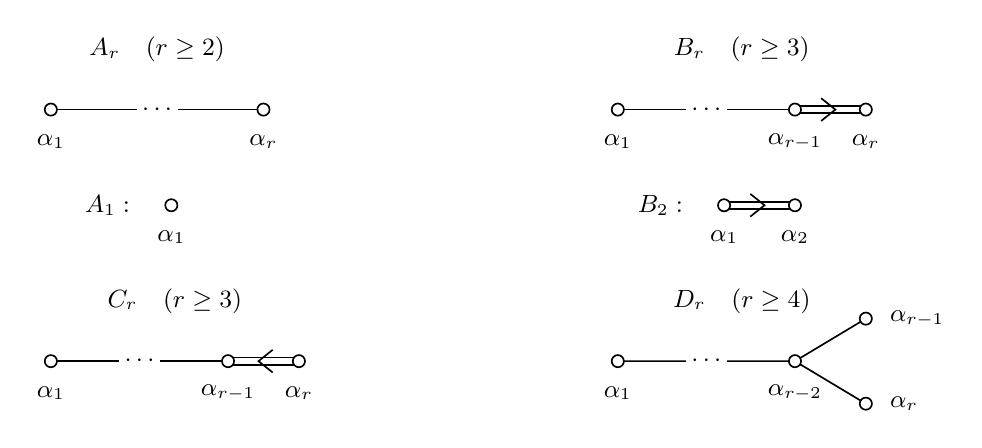
\begin{tikzpicture}[
  x=0.9cm,y=0.9cm,every node/.style={font=\small},
  every path/.style={line width=.6pt},
  root/.style={circle,draw,fill=white,inner sep=0pt,minimum size=4.4pt}]
  % A_r: the omitted single-edge chain may have no intermediate vertices.
  \node at (1.5,0.85) {\(A_r\quad(r\geq2)\)};
  \draw (0,0)--(3,0);
  \node[fill=white,inner sep=2pt] at (1.5,0) {\(\cdots\)};
  \node[root] at (0,0) {};
  \node[root] at (3,0) {};
  \node at (0,-0.45) {\(\alpha_1\)};
  \node at (3,-0.45) {\(\alpha_r\)};
  \node at (0.8,-1.35) {\(A_1:\)};
  \node[root] at (1.7,-1.35) {};
  \node at (1.7,-1.8) {\(\alpha_1\)};

  % B_r: alpha_r is short, so the double-edge arrow points right.
  \node at (9.75,0.85) {\(B_r\quad(r\geq3)\)};
  \draw (8,0)--(10.5,0);
  \node[fill=white,inner sep=2pt] at (9.25,0) {\(\cdots\)};
  \draw (10.5,0.05)--(11.5,0.05) (10.5,-0.05)--(11.5,-0.05);
  \draw (10.87,0.16)--(11.07,0)--(10.87,-0.16);
  \foreach \x in {8,10.5,11.5} \node[root] at (\x,0) {};
  \node at (8,-0.45) {\(\alpha_1\)};
  \node at (10.5,-0.45) {\(\alpha_{r-1}\)};
  \node at (11.5,-0.45) {\(\alpha_r\)};
  \node at (8.6,-1.35) {\(B_2:\)};
  \draw (9.5,-1.3)--(10.5,-1.3) (9.5,-1.4)--(10.5,-1.4);
  \draw (9.87,-1.19)--(10.07,-1.35)--(9.87,-1.51);
  \foreach \x in {9.5,10.5} \node[root] at (\x,-1.35) {};
  \node at (9.5,-1.8) {\(\alpha_1\)};
  \node at (10.5,-1.8) {\(\alpha_2\)};

  % C_r: alpha_r is long, so the double-edge arrow points left.
  \node at (1.75,-2.7) {\(C_r\quad(r\geq3)\)};
  \draw (0,-3.55)--(2.5,-3.55);
  \node[fill=white,inner sep=2pt] at (1.25,-3.55) {\(\cdots\)};
  \draw (2.5,-3.5)--(3.5,-3.5) (2.5,-3.6)--(3.5,-3.6);
  \draw (3.13,-3.39)--(2.93,-3.55)--(3.13,-3.71);
  \foreach \x in {0,2.5,3.5} \node[root] at (\x,-3.55) {};
  \node at (0,-4) {\(\alpha_1\)};
  \node at (2.5,-4) {\(\alpha_{r-1}\)};
  \node at (3.5,-4) {\(\alpha_r\)};

  % D_r: alpha_{r-2} is the fork; at r=4 the omitted chain is one edge.
  \node at (9.75,-2.7) {\(D_r\quad(r\geq4)\)};
  \draw (8,-3.55)--(10.5,-3.55)
    (10.5,-3.55)--(11.5,-2.95) (10.5,-3.55)--(11.5,-4.15);
  \node[fill=white,inner sep=2pt] at (9.25,-3.55) {\(\cdots\)};
  \foreach \x/\y in {8/-3.55,10.5/-3.55,11.5/-2.95,11.5/-4.15}
    \node[root] at (\x,\y) {};
  \node at (8,-4) {\(\alpha_1\)};
  \node at (10.5,-4) {\(\alpha_{r-2}\)};
  \node[anchor=west] at (11.7,-2.95) {\(\alpha_{r-1}\)};
  \node[anchor=west] at (11.7,-4.15) {\(\alpha_r\)};
\end{tikzpicture}
\caption[经典型 Dynkin 图]{经典型 Dynkin 图。省略号表示可含零个中间顶点的单边链段，根的编号沿链递增。
双边箭头指向短根；\(D_r\) 的分叉点为 \(\alpha_{r-2}\)。}
\label{b5:fig:classical-dynkin-diagrams}
\end{figure}
